\begin{auf}
    620
\end{auf}
Zwischen den übereinander liegenden Polen eines Hufeisenmagneten befindet sich, an dünnen Stromzuführungen waagrecht aufgehängt, ein Draht aus Aluminium (Dichte $\varrho=2.7\cdot10\frac{kg}{m^3}$), welcher im vertikalen Magnetfeld (Flussdichte $B=0.08 T$) frei schwingen kann. Durch den Draht fließt ein Strom der Stromdichte $j=10^5\frac{A}{m^2}$. Um welchen Winkel $\varphi$ gegenüber der Senkrechten wird die Pendelaufhängung (sog. LORENTZ-Schaukel) ausgelenkt?
\begin{figure}[h]
    \centering
    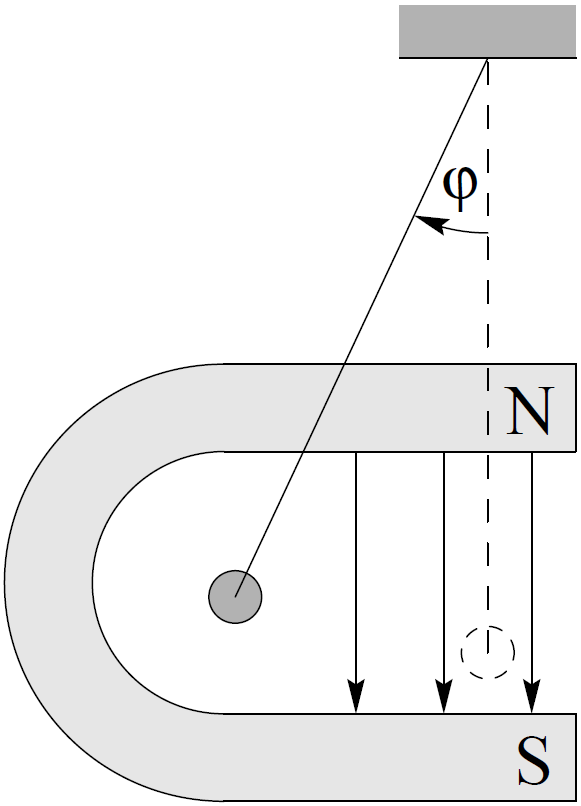
\includegraphics[height=5cm]{images/620_0.png}
    \caption{Versuchsaufbau Aufgabe 620}
\end{figure}